\textbf{so} Text \textit{schreiben} asdfigdfs;oijgs;oef.

sadfasfdas ldfas dlfj asldfnasdfasl

	\begin{figure}[ht]
		\centering
		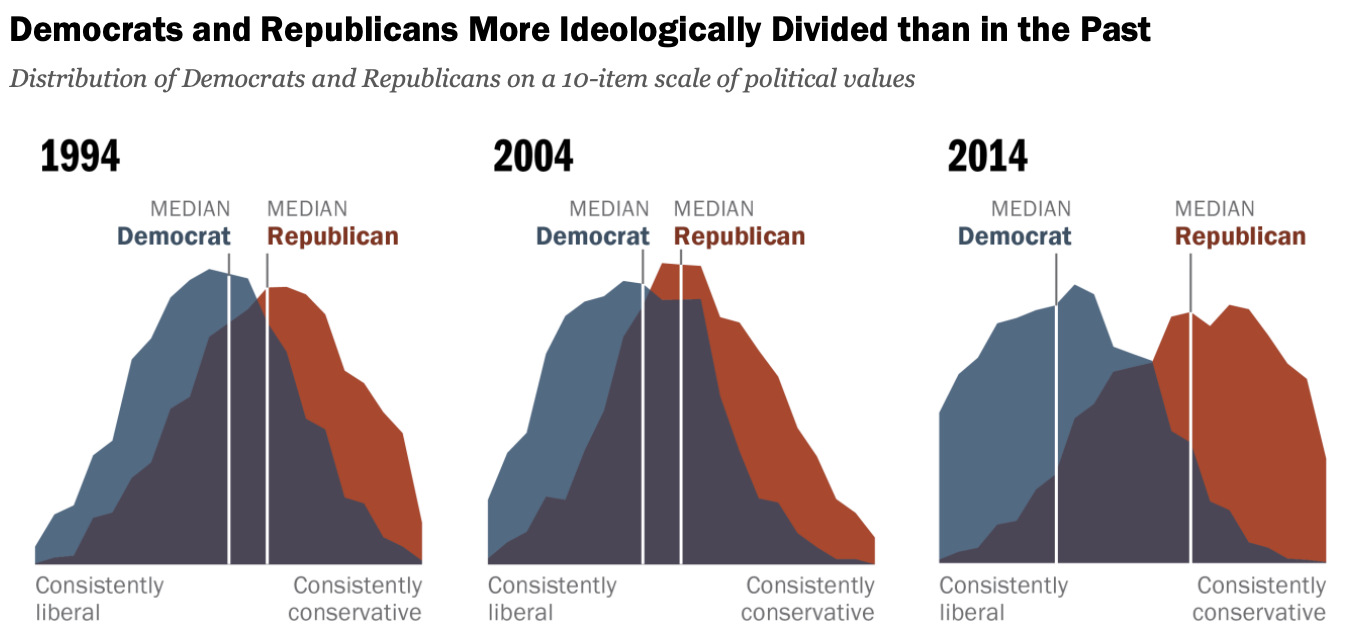
\includegraphics[width=0.9\textwidth]{images/Kapitel1/PoliticalPolarization}
		\captionof{figure}{Ine Beschreibung f}
	\end{figure}
	

{figureBild}

Hier kommt der Text hin.

Zitiere \citeint{dartMouth} Internetverzeichnis.

Oder zitiere \citelit{politicalPolarization} Literaturverzeichnis.